% -*- fill-column: 80 -*-

\documentclass[11pt,a4paper]{article}

\usepackage[margin=2.5cm]{geometry}
\usepackage[dvipsnames]{xcolor}
\usepackage{todonotes}
\usepackage{microtype}
\usepackage{amssymb,amsmath}
\usepackage{mathpazo}
\usepackage{longtable,booktabs}
\usepackage{dcolumn}
\usepackage{graphicx}
\usepackage{natbib}
\usepackage{hyperref}
\usepackage[capitalise,noabbrev,nameinlink]{cleveref}
\hypersetup{
  pdftitle={Ouroboros Leios simulation: building confidence in the performance results},
  pdfborder={0 0 0},
  breaklinks=true
}
\usepackage{subcaption}
\usepackage{listings}
%%\newcommand{\debug}[1]{}
\newcommand{\debug}[1]{#1}
\newcommand{\scenarioVsIdealFigure}[2]{
\begin{figure}[htbp]
    \centering
    \debug{\textbf{Label: #2} \\}
    \begin{subfigure}[b]{0.45\textwidth}
        \centering
        \includegraphics[width=\textwidth]{{#1}/IB-0.5-vs-ideal-vs-fitted-fig.eps}
        \caption{IB diffusion to $0.50$ stake.}
        \label{#1:ib0.5}
    \end{subfigure}
    \hfill
    \begin{subfigure}[b]{0.45\textwidth}
        \centering
        \includegraphics[width=\textwidth]{{#1}/IB-0.98-vs-ideal-vs-fitted-fig.eps}
        \caption{IB diffusion to $0.98$ stake.}
        \label{#1:ib0.98}
    \end{subfigure}
    
    \vspace{1em}
    
    \begin{subfigure}[b]{0.45\textwidth}
        \centering
        \includegraphics[width=\textwidth]{{#1}/EB-0.5-vs-ideal-vs-fitted-fig.eps}
        \caption{EB diffusion to $0.50$ stake.}
        \label{#1:eb0.5}
    \end{subfigure}
    \hfill
    \begin{subfigure}[b]{0.45\textwidth}
        \centering
        \includegraphics[width=\textwidth]{{#1}/EB-0.98-vs-ideal-vs-fitted-fig.eps}
        \caption{EB diffusion to $0.98$ stake.}
        \label{#1:eb0.98}
    \end{subfigure}
    
    \vspace{1em}
    
    \begin{subfigure}[b]{0.45\textwidth}
        \centering
        \includegraphics[width=\textwidth]{{#1}/VT-0.5-vs-ideal-vs-fitted-fig.eps}
        \caption{VT diffusion to $0.50$ stake.}
        \label{#1:vt0.5}
    \end{subfigure}
    \hfill
    \begin{subfigure}[b]{0.45\textwidth}
        \centering
        \includegraphics[width=\textwidth]{{#1}/VT-0.98-vs-ideal-vs-fitted-fig.eps}
        \caption{VT diffusion to $0.98$ stake.}
        \label{#1:vt0.98}
    \end{subfigure}
    
    \vspace{1em}
    
    \begin{subfigure}[b]{0.45\textwidth}
        \centering
        \includegraphics[width=\textwidth]{{#1}/RB-0.5-vs-ideal-vs-fitted-fig.eps}
        \caption{RB diffusion to $0.50$ stake.}
        \label{#1:rb0.5}
    \end{subfigure}
    \hfill
    \begin{subfigure}[b]{0.45\textwidth}
        \centering
        \includegraphics[width=\textwidth]{{#1}/RB-0.98-vs-ideal-vs-fitted-fig.eps}
        \caption{RB diffusion to $0.98$ stake.}
        \label{#1:rb0.98}
    \end{subfigure}

    \caption{Scenario \ref{#2}, diffusion latencies from slot start (300s run with default seed).}
    \label{fig:#1}
\end{figure}
}


\begin{document}

\title{Ouroboros Leios simulation: \\
       building confidence in the performance results \\
       {\large \sc An IOHK technical report}
  }
\date{Version 1.0, April 2021}
\author{Andrea Vezzosi     \\ {\small \texttt{andrea@well-typed.com}} \\
   \and Wen Kokke          \\ {\small \texttt{wen@well-typed.com}} \\
   \and Duncan Coutts      \\ {\small \texttt{duncan@well-typed.com}}
   }

\maketitle

\section{Introduction}
\label{introduction}


\tableofcontents

\listoftodos

\section{Summary}
\label{summary}

Most idealized setting for the simulation:
\begin{itemize}
\item Nodes request block bodies from every peer.
\item Mini-protocols are each run on a dedicated connection.
\item The network model is a simplified one where packets are sent in-order and
  limited only by latency and bandwidth.
\item An unbounded number of CPU intensive tasks, like validation, are simulated to run in parallel.
\item Delays and sizes for blocks are kept uniform.
\end{itemize}

Scenarios proceed from most idealized and gradually turn one more realism feature:
\begin{enumerate}
\item \label{sc:most-idealized} most idealized.
\item \label{sc:request-from-first} nodes request block bodies from first peer available.
\item \label{sc:multiplexing} mini-protocols are multiplexed over one connection.
\item \label{sc:tcp} network layer more closely models TCP, in particular acks
  and congestion window collapse/restart.
\item \label{sc:boundedcpu} nodes simulate CPU tasks with a finite number of worker threads.
\item \label{sc:order} request IB bodies in oldest-first order.
\end{enumerate}
The last scenario is not strictly about realism, but we rather want to
investigate the impact of deviating from the freshest-first default.

\section{Scenario \ref{sc:most-idealized}}
\label{scenario1}
The least realistic scenario. Config:
\lstinputlisting[firstline=7]{scenario1/config.yaml}
\todo{remove config once scenario explained}

In Figure~\ref{fig:scenario1} we compute ideal times two ways:
\begin{itemize}
\item \textbf{ideal} -- Uses $3$ latencies for every communication.
\item \textbf{ideal-fitted} -- Uses $3$ latencies for RB and EB, but $4$ for IB and $3.5$ for Votes.
\end{itemize}
we see that ideal-fitted better matches the simulation.

The Relay mini-protocol involves the consumer first requesting new headers, so
it can take $4$ latencies to receive the body. When blocks are more sporadic,
like for EBs and RBs, the consumer has likely already sent a blocking request
for more headers, so $3$ latencies are enough.
Votes all get sent at the start of the slice, with default configuration at least, so we can expect consumers to reach the blocking stage again by the next burst. However, due to the large traffic, the $4$ latencies path likely sees some use too. This mix of behaviours can explain the better fit using $3.5$ latencies.

\scenarioVsIdealFigure{scenario1}{sc:most-idealized}

\subsection{Uniform Voting stage}
The diffusion latencies, in Fig. \ref{fig:scenario1-send-recv}, stay very
similar when the simulation is set to generate votes across the whole stage
rather than only in the first slot.
From second $80$ to $300$ we have $\sim 1100$ vote messages, for an average of $\sim 5$
VT/s, same as IBs. The traffic pattern then does not seem a factor in the observed behaviour.
\begin{figure}[htbp]
    \centering
    \begin{subfigure}[b]{0.45\textwidth}
        \centering
        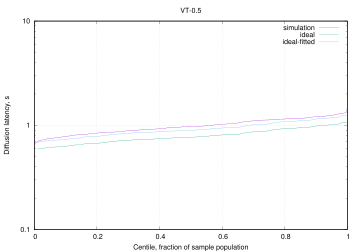
\includegraphics[width=\textwidth]{scenario1/VT-0.5-vs-ideal-vs-fitted-fig.eps}
        \caption{VT diffusion to $0.50$ stake.}
        \label{scenario1-send-recv:vt0.5}
    \end{subfigure}
    \hfill
    \begin{subfigure}[b]{0.45\textwidth}
        \centering
        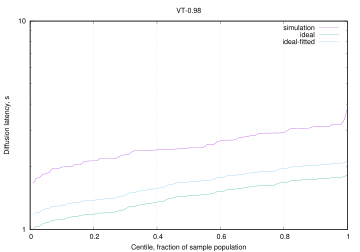
\includegraphics[width=\textwidth]{scenario1/VT-0.98-vs-ideal-vs-fitted-fig.eps}
        \caption{VT diffusion to $0.98$ stake.}
        \label{scenario1-send-recv:vt0.98}
    \end{subfigure}
    \caption{Scenario \ref{sc:most-idealized} with \textbf{uniform voting}, diffusion latencies from slot start (300s run with default seed).}
    \label{fig:scenario1-send-recv}
\end{figure}

\subsection{Large votes}
The diffusion latencies, in Fig. \ref{fig:scenario1-big-votes} and
\ref{fig:scenario1-big-votes-send-recv}, are collected for votes set to the size
of input blocks. With start-of-stage voting (the default) we see diffusion running
slightly slower than ideal with $4$ latencies, while uniform voting has a very
close fit. The delay in the former is possibly due to the $\sim 0.05s$
serialization time causing blocks to queue behind each other when they are all
generated at once: the volume of data, $102400*100$, is $5$ times the bandwidth
of any given link, and nodes are requesting bodies from everyone.

\begin{figure}[htbp]
    \centering
    \begin{subfigure}[b]{0.45\textwidth}
        \centering
        \includegraphics[width=\textwidth]{scenario1-big-votes/VT-0.5-vs-ideal-4-hops-fig.eps}
        \caption{VT diffusion to $0.50$ stake.}
        \label{scenario1-big-votes:vt0.5}
    \end{subfigure}
    \hfill
    \begin{subfigure}[b]{0.45\textwidth}
        \centering
        \includegraphics[width=\textwidth]{scenario1-big-votes/VT-0.98-vs-ideal-4-hops-fig.eps}
        \caption{VT diffusion to $0.98$ stake.}
        \label{scenario1-big-votes:vt0.98}
    \end{subfigure}
    \caption{Scenario \ref{sc:most-idealized} with \textbf{large votes, start-of-stage voting}, diffusion latencies from slot start (300s run with default seed).}
    \label{fig:scenario1-big-votes}
\end{figure}
\begin{figure}[htbp]
    \centering
    \begin{subfigure}[b]{0.45\textwidth}
        \centering
        \includegraphics[width=\textwidth]{scenario1-big-votes-send-recv/VT-0.5-vs-ideal-4-hops-fig.eps}
        \caption{VT diffusion to $0.50$ stake.}
        \label{scenario1-big-votes-send-recv:vt0.5}
    \end{subfigure}
    \hfill
    \begin{subfigure}[b]{0.45\textwidth}
        \centering
        \includegraphics[width=\textwidth]{scenario1-big-votes-send-recv/VT-0.98-vs-ideal-4-hops-fig.eps}
        \caption{VT diffusion to $0.98$ stake.}
        \label{scenario1-big-votes-send-recv:vt0.98}
    \end{subfigure}
    \caption{Scenario \ref{sc:most-idealized} with \textbf{large votes, uniform voting}, diffusion latencies from slot start (300s run with default seed).}
    \label{fig:scenario1-big-votes-send-recv}
\end{figure}

\section{Scenario \ref{sc:request-from-first}}
\label{scenario2}
Fig.~\ref{fig:scenario2}
\scenarioVsIdealFigure{scenario2}{sc:request-from-first}
\todo{compare to previous plot rather than ideal? Same for later sections.}

\section{Scenario \ref{sc:multiplexing}}
\label{scenario3}
Fig.~\ref{fig:scenario3}
\scenarioVsIdealFigure{scenario3}{sc:multiplexing}

\section{Scenario \ref{sc:tcp}}
\label{scenario4}
Fig.~\ref{fig:scenario4}
\scenarioVsIdealFigure{scenario4}{sc:tcp}
\todo{do IBs which do not reference RBs do better?}

\todo{clarify each scenario variation}
scenario4-best-IB-rate Fig.~\ref{fig:scenario4-best-IB-rate}
\scenarioVsIdealFigure{scenario4-best-IB-rate}{sc:tcp-opt}

scenario4-higher-IB-rate Fig.~\ref{fig:scenario4-higher-IB-rate}
\scenarioVsIdealFigure{scenario4-higher-IB-rate}{sc:tcp-higher-IB-rate}
\todo{Use send-recv to see if voting diffusion improves with this much traffic}

scenario4-lower-stage-length Fig.~\ref{fig:scenario4-lower-stage-length}
\scenarioVsIdealFigure{scenario4-lower-stage-length}{sc:tcp-lower-stage-length}
\todo{Try reducing validation times for IBs}


scenario4-20IB-small Fig.~\ref{fig:scenario4-20IB-small}
\scenarioVsIdealFigure{scenario4-20IB-small}{sc:tcp-20IB-small}

\section{Scenario \ref{sc:boundedcpu}}
\label{scenario5}
Fig.~\ref{fig:scenario5}
\scenarioVsIdealFigure{scenario5}{sc:boundedcpu}

\section{Scenario \ref{sc:order}}
\label{scenario6}
Fig.~\ref{fig:scenario6}
\scenarioVsIdealFigure{scenario6}{sc:order}

Fix.~\ref{fig:oldest-vs-freshest}
\begin{figure}[htbp]
    \centering
    \debug{\textbf{Label: oldest-vs-freshest} \\}
    \begin{subfigure}[b]{0.45\textwidth}
        \centering
        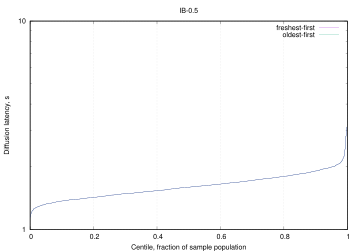
\includegraphics[width=\textwidth]{scenario6/IB-0.5-oldest-vs-freshest.eps}
        \caption{IB diffusion to $0.50$ stake.}
        \label{fig:oldest-vs-freshest:ib0.5}
    \end{subfigure}
    \hfill
    \begin{subfigure}[b]{0.45\textwidth}
        \centering
        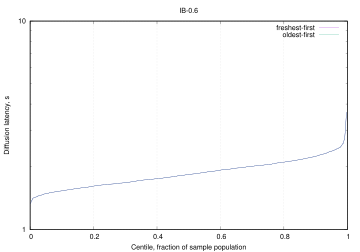
\includegraphics[width=\textwidth]{scenario6/IB-0.6-oldest-vs-freshest.eps}
        \caption{IB diffusion to $0.60$ stake.}
        \label{fig:oldest-vs-freshest:ib0.6}
    \end{subfigure}
    
    \vspace{1em}
    
    \begin{subfigure}[b]{0.45\textwidth}
        \centering
        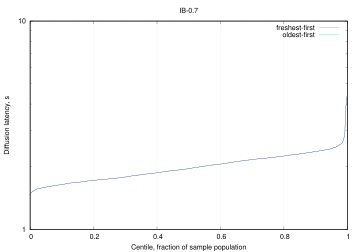
\includegraphics[width=\textwidth]{scenario6/IB-0.7-oldest-vs-freshest.eps}
        \caption{IB diffusion to $0.70$ stake.}
        \label{fig:oldest-vs-freshest:ib0.7}
    \end{subfigure}
    \hfill
    \begin{subfigure}[b]{0.45\textwidth}
        \centering
        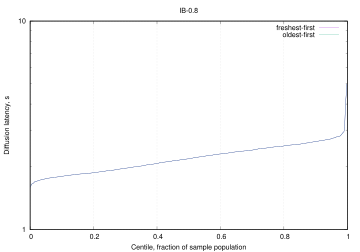
\includegraphics[width=\textwidth]{scenario6/IB-0.8-oldest-vs-freshest.eps}
        \caption{IB diffusion to $0.80$ stake.}
        \label{fig:oldest-vs-freshest:ib0.8}
    \end{subfigure}
    
    \vspace{1em}
    
    \begin{subfigure}[b]{0.45\textwidth}
        \centering
        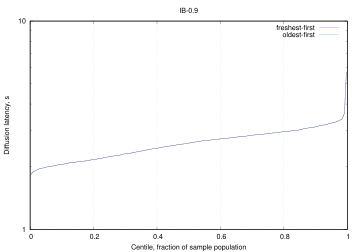
\includegraphics[width=\textwidth]{scenario6/IB-0.9-oldest-vs-freshest.eps}
        \caption{IB diffusion to $0.90$ stake.}
        \label{fig:oldest-vs-freshest:ib0.9}
    \end{subfigure}
    \hfill
    \begin{subfigure}[b]{0.45\textwidth}
        \centering
        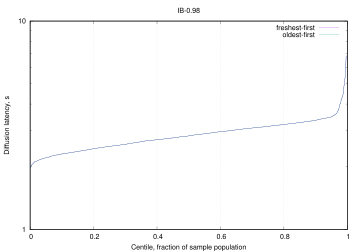
\includegraphics[width=\textwidth]{scenario6/IB-0.98-oldest-vs-freshest.eps}
        \caption{IB diffusion to $0.98$ stake.}
        \label{fig:oldest-vs-freshest:ib0.98}
    \end{subfigure}

    \caption{Scenario \ref{sc:order}, diffusion latencies from slot start (300s run with default seed).}
    \label{fig:oldest-vs-freshest}
\end{figure}


\addcontentsline{toc}{section}{References}
\bibliographystyle{plainnat}
\bibliography{sim-realism}

\end{document}
